\documentclass[11pt]{article}
\usepackage[margin=1in]{geometry}
\usepackage{graphicx}
\usepackage{booktabs}
\usepackage{caption}
\usepackage{subcaption}
\usepackage[table]{xcolor}
\usepackage{amsmath}
\usepackage{hyperref}

\title{HIL Benchmark: ORB-SLAM2 vs.\ OV2SLAM (Accurate)}
\author{ROS2 HIL Visual-Servoing Project}
\date{2026-07-05}

\begin{document}
\maketitle

\section{Summary}

This report compares ORB-SLAM2 and OV2SLAM (accurate profile) on the same
hardware-in-the-loop (HIL) flight scenario: an oracle detector + proportional
controller flying the same approach trajectory, with the \texttt{INITIALIZER\_GATE}
warm-up enabled for both backends. Three repeated runs per backend (run tag
\texttt{preflight\_code\_julien\_\{1,2,3\}}, 2026-07-05) were evaluated by
literally invoking the \texttt{evo\_ape} command-line tool
(\href{https://github.com/MichaelGrupp/evo}{evo}, the same tool the offline
EuRoC benchmark study used) as a subprocess -- \texttt{evo\_ape tum gt.tum
slam.tum --align --correct\_scale} -- and parsing its stdout, not a hand-written
re-implementation of evo's alignment/association code. All accuracy figures are
reported in meters.

\textbf{Both backends tracked the full mission successfully in all 6 runs} --
this is itself a result: OV2SLAM failed to initialize in every attempt prior to
this run (see \texttt{docs/fixlog/014}, \texttt{015} for the diagnosis and fixes
that made this data possible).

\begin{center}
\colorbox{yellow}{%
  \begin{minipage}{0.92\textwidth}
  \textbf{Important -- neither backend is actually flying the drone in these
  runs.} Both configs use \texttt{detector.type: oracle} with
  \texttt{controller.use\_slam\_pose}/\texttt{use\_slam\_depth} left at their
  default (\texttt{false} -- confirmed in \texttt{parse\_stack.py}). The
  proportional controller's control input is the oracle detector's
  ground-truth-derived bounding box (\texttt{/yolo/detections}), not SLAM.
  \textbf{SLAM is a passive passenger here}: recorded and evaluated for
  accuracy, but it never influences \texttt{/cmd\_vel} or the flight path.
  This is the right setup for an apples-to-apples accuracy/performance
  comparison (both backends fly the identical, repeatable, SLAM-independent
  path), but it does \emph{not} demonstrate SLAM-driven visual servoing.
  \end{minipage}%
}
\end{center}

\paragraph{How easy would SLAM-driven control actually be?} For the
\emph{IBVS} controller (TS1), trivially easy -- \texttt{controller.use\_slam\_depth}/
\texttt{use\_slam\_pose} are real, already-implemented parameters
(\texttt{visp\_servo/src/ibvs\_controller.cpp:19-38}), wired all the way from
the stack config through the launch file to the controller (see
\texttt{ov2slam\_ibvs.yaml}); switching to SLAM-driven IBVS is a config change,
not new code (though it inherits known open caveats -- monocular scale drift,
background-vs-target depth bias -- tracked in \texttt{docs/fixlog/009}).
\emph{Not} implemented for the \textbf{proportional controller (TS2)} used in
this report, and there is a concrete reason: TS2's entire control law
(\texttt{proportional\_controller.cpp:29-41}) is 2D image-plane only -- forward
velocity from apparent bounding-box size, lateral/vertical velocity from
normalised pixel offset. It never needs depth or 3D pose at all, unlike IBVS's
image Jacobian, which requires an explicit depth estimate. Wiring SLAM into TS2
wouldn't extend it so much as replace its control law with something closer to
PBVS (TS4) -- a materially different controller, not a flag flip. Separately:
"oracle" and "TS2" are independent axes (detector choice vs.\ controller
choice) that already compose freely -- oracle+proportional is exactly what
this report benchmarks; there is no such thing as an "oracle controller."

\section{ATE RMSE and Tracking Coverage}

Two ATE numbers are reported per run. \textbf{Mission ATE} restricts evaluation
to $t \geq$ FSM-start (the \texttt{/bench/state} marker), excluding the
\texttt{INITIALIZER\_GATE}'s own pre-mission warm-up wiggle -- this is the number
that reflects actual tracking quality during the flight, and the one used for
comparison. \textbf{Full-bag ATE} includes that warm-up window too, for
transparency; it reads noticeably higher because a handful of high-error points
right after SLAM initializes (before scale/pose has settled) get squared into
the RMSE despite being a small fraction of the total samples -- see the note at
the end of this section for the concrete numbers behind that gap.

\emph{Sample size caveat}: \texttt{evo\_ape}'s own default association tolerance
(\texttt{--t\_max\_diff 0.01}s) is tight relative to GT's $\sim$50\,Hz and SLAM's
$\sim$16--20\,Hz rates, so only pose pairs within 10\,ms of each other count --
between 32 and 171 pairs per run here (out of hundreds of raw samples each). This
is \texttt{evo\_ape}'s real default, used deliberately instead of a looser
custom tolerance (see the summary above), but it does mean each run's RMSE
reflects a sparser sample than the raw pose counts might suggest.

``GT\%'' is \texttt{slam\_coverage\_after\_fsm\_pct} -- the SLAM-estimated path
length (scaled by the Umeyama factor) divided by the ground-truth path length
flown after FSM start. A value near 100\% means the backend tracked essentially
the whole mission at the correct scale; a value far below 100\% would indicate
it lost tracking partway through despite a low RMSE.

\begin{table}[h]
\centering
\caption{ATE RMSE (mission-only, primary; full-bag, for reference) and tracking coverage, per run and aggregated (mean $\pm$ std across the 3 runs).}
\label{tab:ate}
\begin{tabular}{llrrr}
\toprule
Algorithm & Run & Mission ATE (m) & Full-bag ATE (m) & GT\% (coverage) \\
\midrule
ORB-SLAM2 & julien\_1 & 0.1263 & 0.1661 & 112.00\% \\
ORB-SLAM2 & julien\_2 & 0.1815 & 0.1896 & 110.77\% \\
ORB-SLAM2 & julien\_3 & 0.1231 & 0.1231 & 106.20\% \\
\textbf{ORB-SLAM2} & \textbf{mean $\pm$ std} & \textbf{0.1436 $\pm$ 0.0328} & \textbf{0.1596 $\pm$ 0.0337} & \textbf{109.66\% $\pm$ 3.06\%} \\
\addlinespace
OV2SLAM (accurate) & julien\_1 & 0.0555 & 0.1087 & 101.17\% \\
OV2SLAM (accurate) & julien\_2 & 0.0617 & 0.1389 & 100.24\% \\
OV2SLAM (accurate) & julien\_3 & 0.0224 & 0.0393 & 101.57\% \\
\textbf{OV2SLAM (accurate)} & \textbf{mean $\pm$ std} & \textbf{0.0465 $\pm$ 0.0211} & \textbf{0.0956 $\pm$ 0.0511} & \textbf{100.99\% $\pm$ 0.68\%} \\
\bottomrule
\end{tabular}
\end{table}

\begin{figure}[h]
\centering
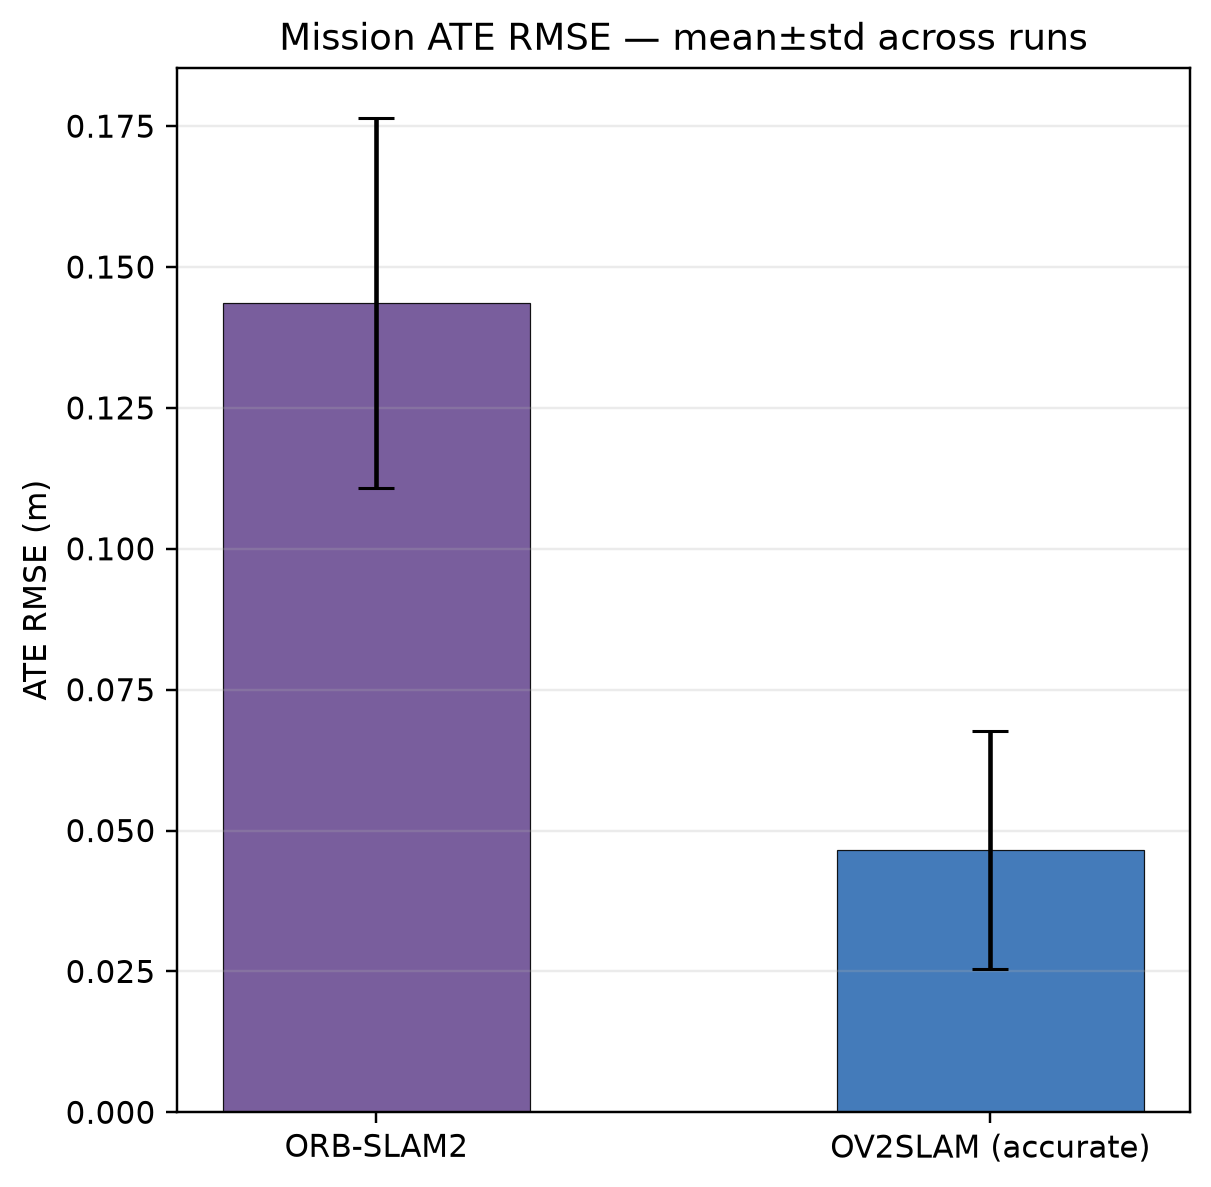
\includegraphics[width=0.75\textwidth]{figures/cmp_ate_rmse.png}
\caption{Mission ATE RMSE, mean $\pm$ std across the 3 runs per backend.}
\label{fig:ate_rmse}
\end{figure}

On mission ATE, OV2SLAM is substantially tighter than ORB-SLAM2 (0.047m vs.\
0.144m mean -- roughly 3$\times$) on this platform, though both show real
run-to-run spread (std 0.021m and 0.033m respectively) given only 3 runs and
the small per-run association counts noted above. OV2SLAM's coverage is also
tighter around 100\% (std 0.68 pts vs.\ 3.06 pts) -- ORB-SLAM2's coverage
exceeding 100\% by more (106--112\%) suggests its scaled trajectory slightly
overshoots the true path length, more so than OV2SLAM's.

\paragraph{Why full-bag ATE reads higher.} Diagnosed concretely on ORB-SLAM2
julien\_1's raw (unassociated) pose stream: the first 20 of 886 raw SLAM poses
average 0.337m error against the nearest GT sample; the remaining 866 average
0.104m. Checking the raw ground truth in that early window: \texttt{x} sits at
exactly \texttt{0.000} throughout while \texttt{y} swings -- i.e.\ this is the
gate's lateral left/right warm-up legs (a purely 2D wiggle near the start
position), not the mission's smooth diagonal approach, and it shows up as a
short near-vertical segment at the start of the full trajectory plots in
Figure~\ref{fig:traj_grid}. SLAM's pose estimate is naturally noisier in this
window (only just initialized, scale/pose not yet settled), so this short
segment contributes disproportionately to a whole-bag RMSE -- which is exactly
why the mission-windowed number above is the one to trust.

\section{Front-End Latency}

\begin{table}[h]
\centering
\caption{Front-end tracking latency per frame, per run and aggregated.}
\label{tab:frontend}
\begin{tabular}{llrr}
\toprule
Algorithm & Run & Mean (ms) & Std (ms) \\
\midrule
ORB-SLAM2 & julien\_1 & 26.902 & 5.052 \\
ORB-SLAM2 & julien\_2 & 24.191 & 3.396 \\
ORB-SLAM2 & julien\_3 & 25.857 & 4.764 \\
\textbf{ORB-SLAM2} & \textbf{mean $\pm$ std across runs} & \textbf{25.650} & \textbf{1.367} \\
\addlinespace
OV2SLAM (accurate) & julien\_1 & 8.298 & 3.289 \\
OV2SLAM (accurate) & julien\_2 & 8.807 & 3.120 \\
OV2SLAM (accurate) & julien\_3 & 7.401 & 2.907 \\
\textbf{OV2SLAM (accurate)} & \textbf{mean $\pm$ std across runs} & \textbf{8.169} & \textbf{0.712} \\
\bottomrule
\end{tabular}
\end{table}

\begin{figure}[h]
\centering
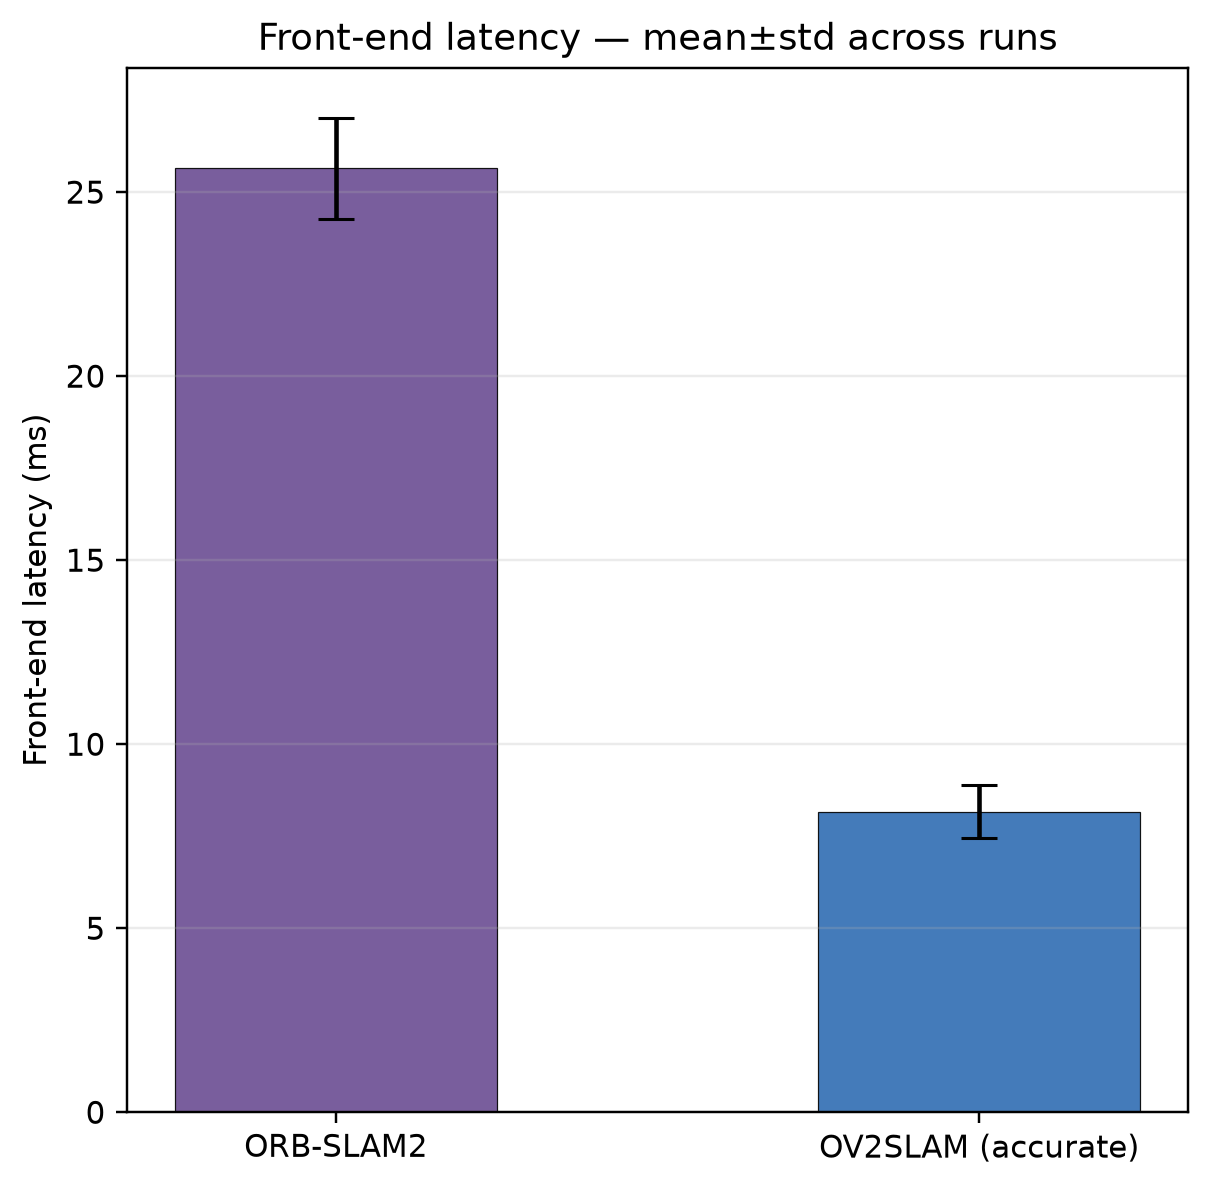
\includegraphics[width=0.75\textwidth]{figures/cmp_frontend_latency.png}
\caption{Front-end tracking latency, mean $\pm$ std across the 3 runs per backend.}
\label{fig:frontend}
\end{figure}

OV2SLAM's front-end is roughly 3$\times$ faster per frame than ORB-SLAM2's on
this platform (8.2\,ms vs.\ 25.7\,ms mean).

\section{CPU Utilization}

\begin{figure}[h]
\centering
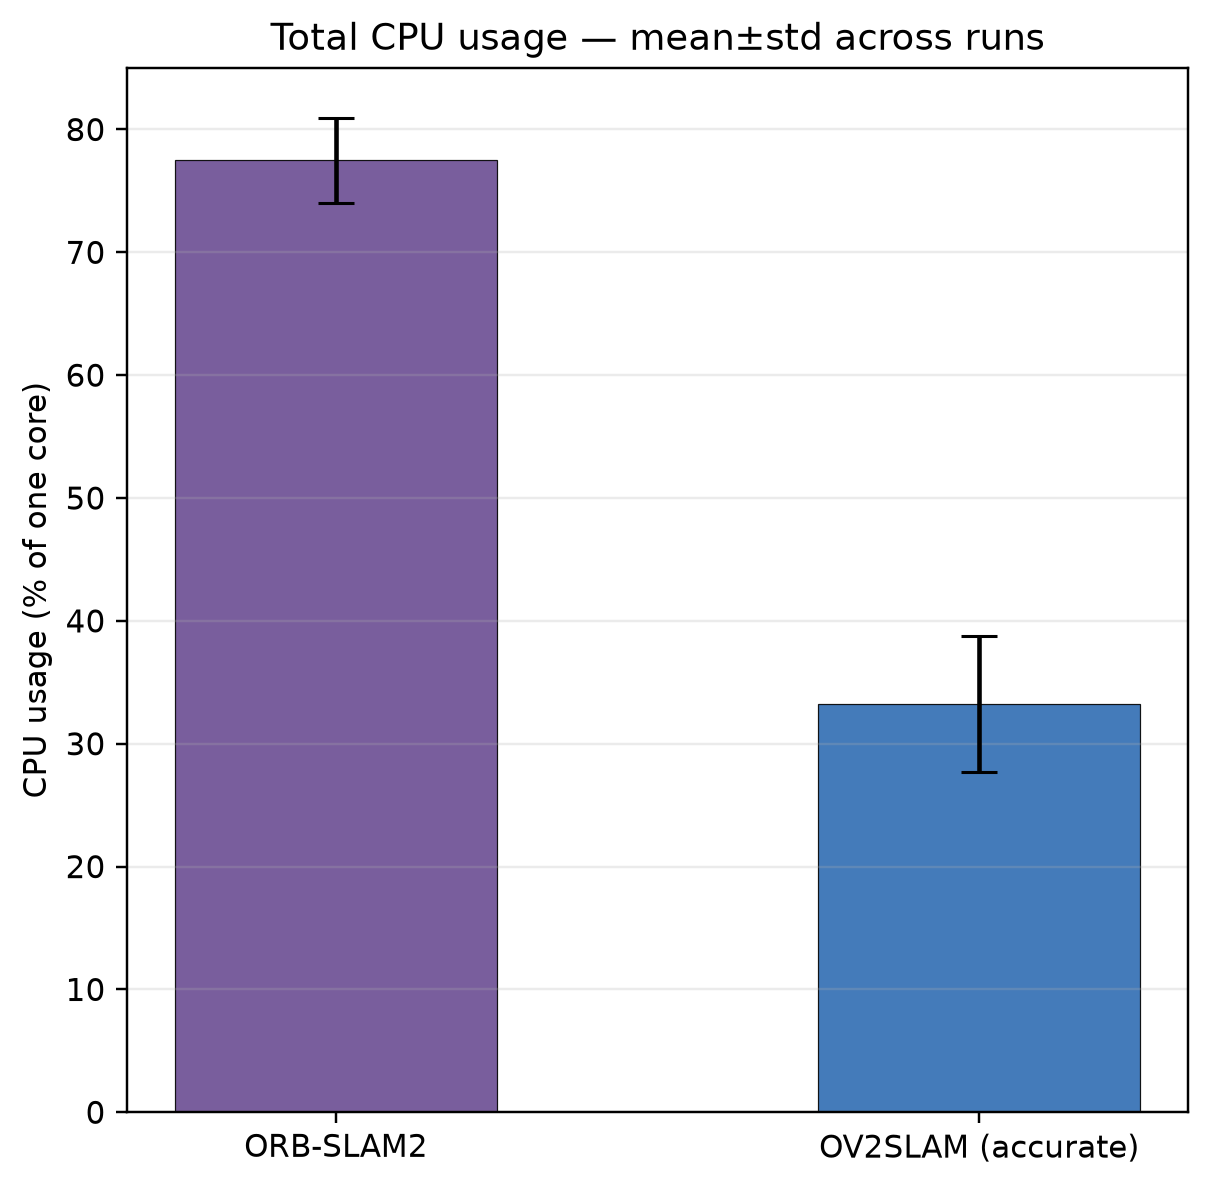
\includegraphics[width=0.75\textwidth]{figures/cmp_cpu_total.png}
\caption{Total process CPU utilization (\% of one core), mean $\pm$ std across the 3 runs per backend.}
\label{fig:cpu_total}
\end{figure}

Total CPU usage follows the same pattern as latency: OV2SLAM uses roughly
less than half the CPU of ORB-SLAM2 on average (33\% vs.\ 77\% of one core).

\section{Per-Thread CPU Breakdown}

\begin{figure}[h]
\centering
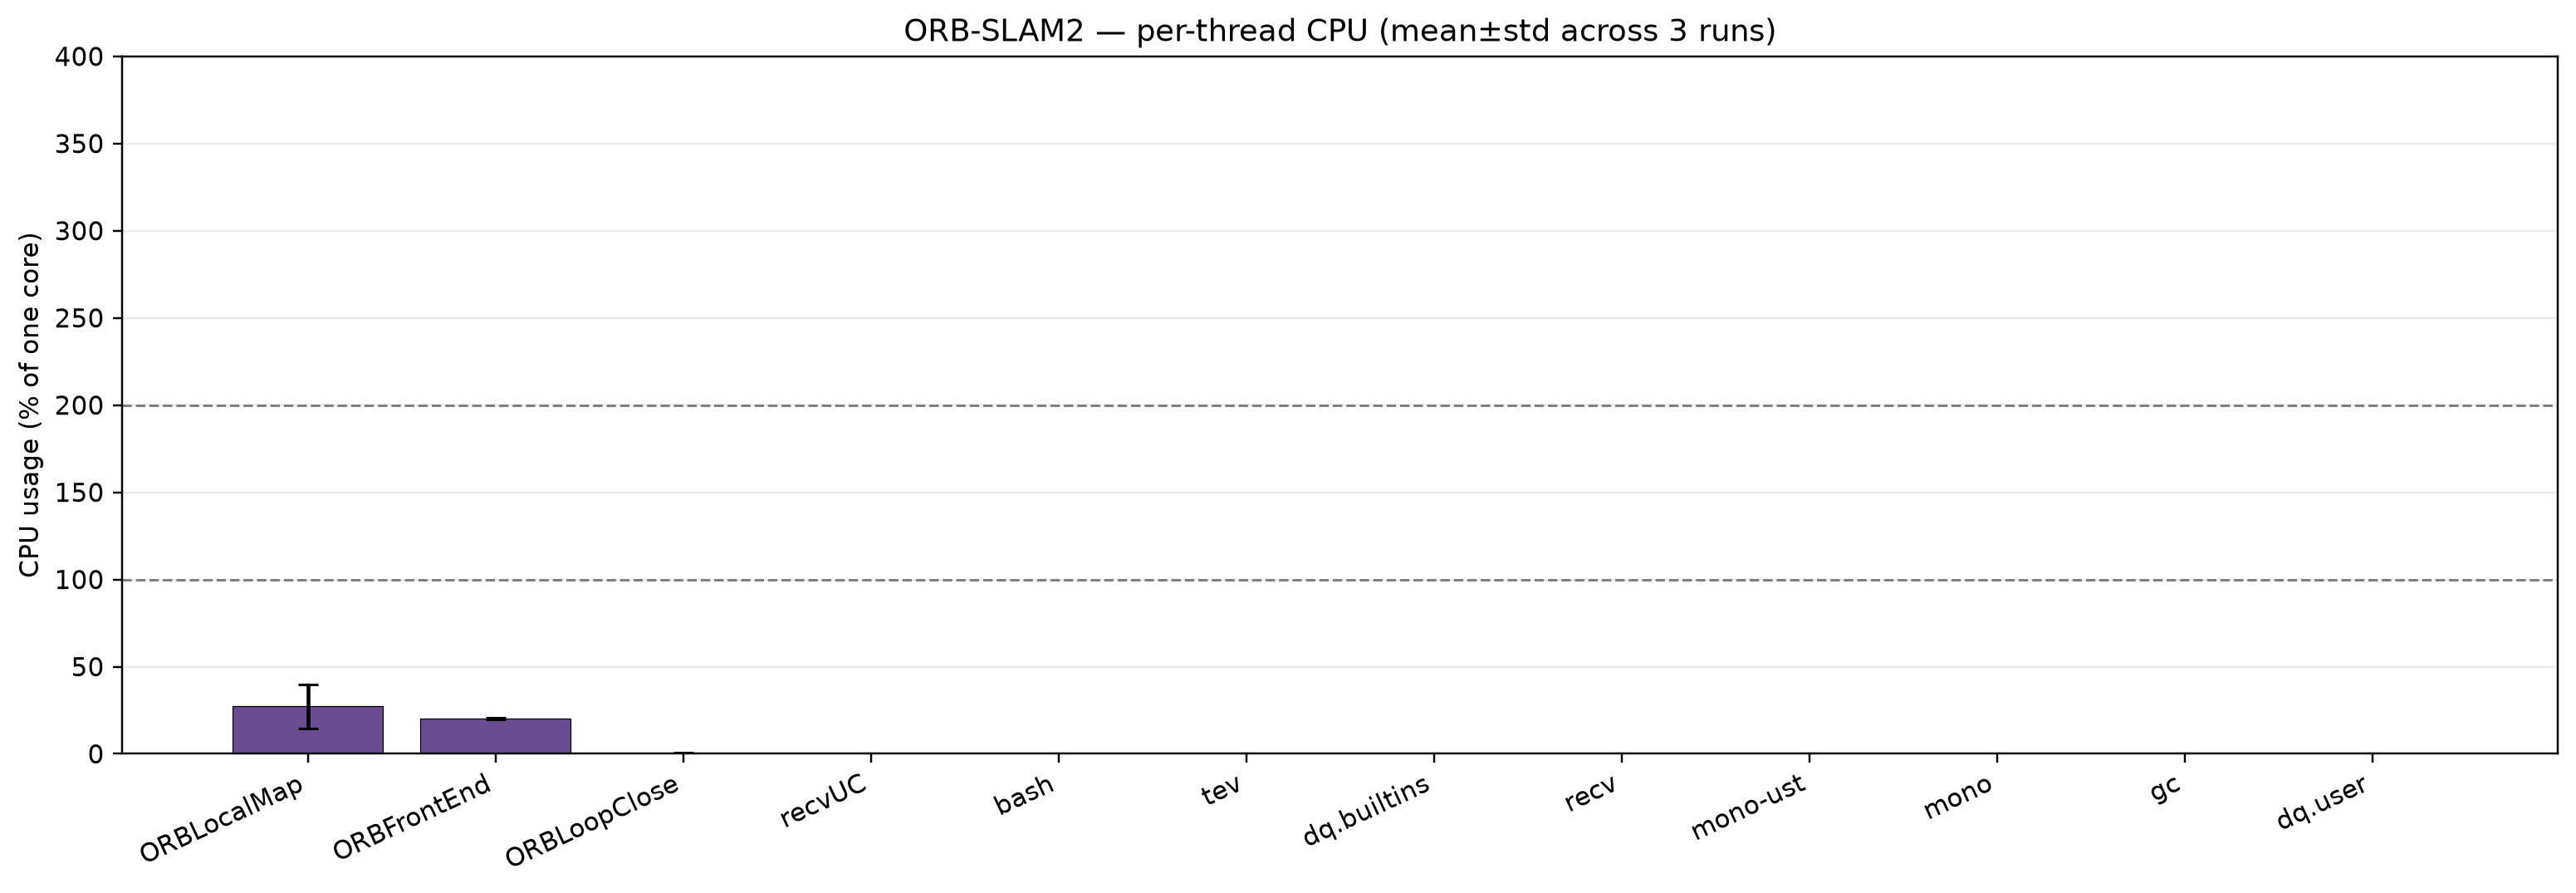
\includegraphics[width=0.95\textwidth]{figures/cmp_thread_orb-slam2.png}
\caption{ORB-SLAM2 per-thread CPU usage, mean $\pm$ std across the 3 runs.
Named internal roles (\texttt{ORBLocalMap}, \texttt{ORBFrontEnd}, \texttt{ORBLoopClose})
dominate; remaining entries are generic OS/runtime threads.}
\label{fig:thread_orb}
\end{figure}

\begin{figure}[h]
\centering
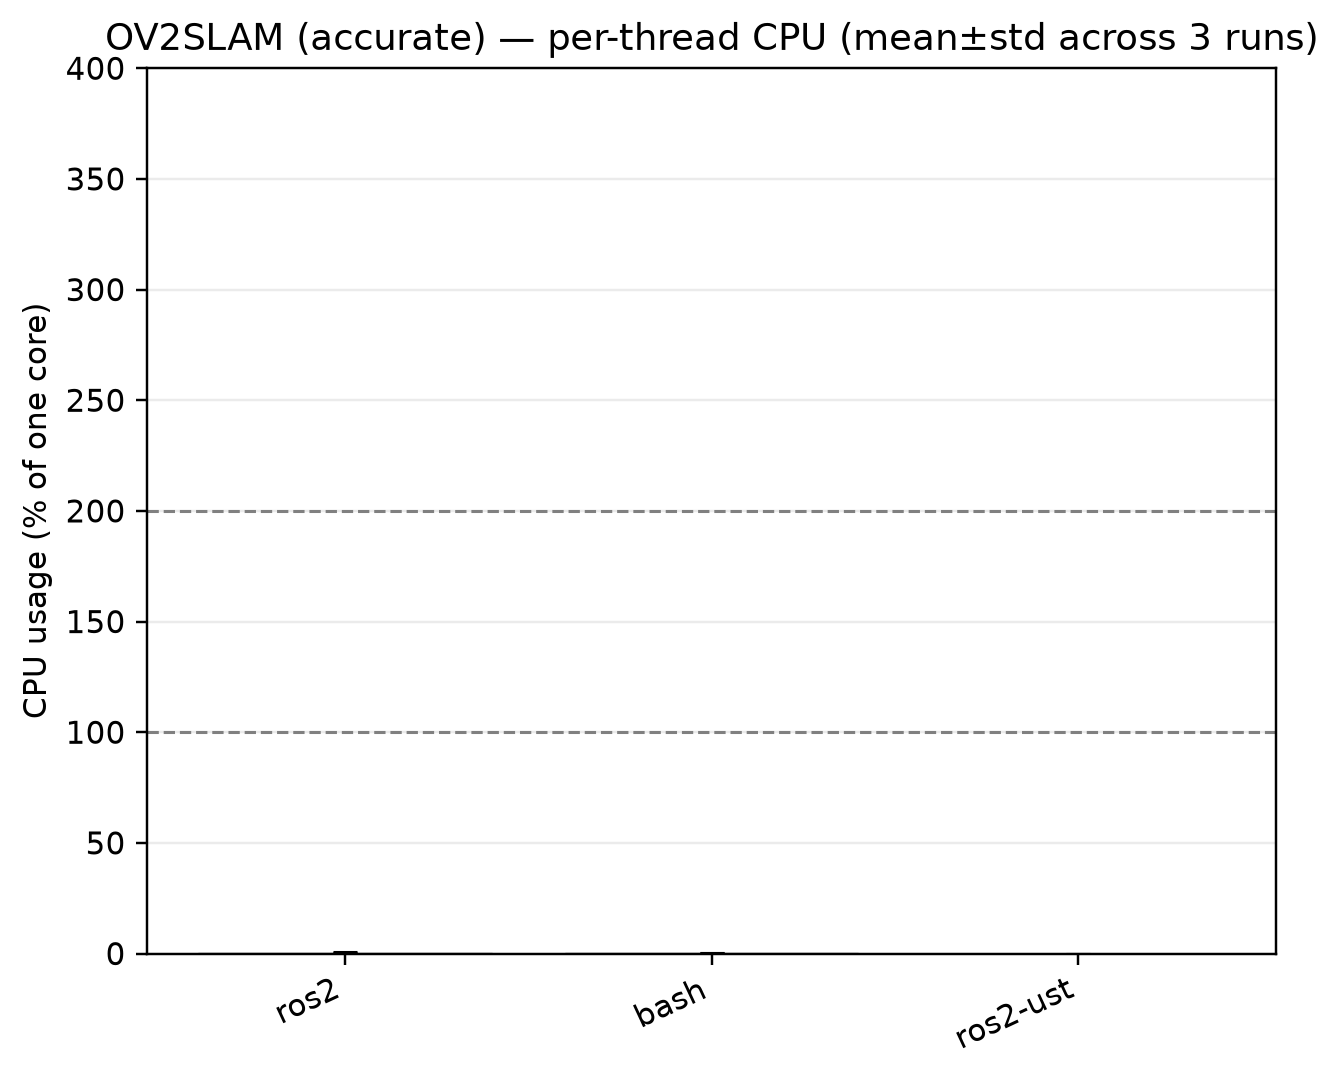
\includegraphics[width=0.95\textwidth]{figures/cmp_thread_ov2slam_accurate.png}
\caption{OV2SLAM per-thread CPU usage as captured in these 3 runs.}
\label{fig:thread_ov2}
\end{figure}

\begin{center}
\colorbox{yellow}{%
  \begin{minipage}{0.92\textwidth}
  \textbf{Data gap -- Figure~\ref{fig:thread_ov2} does not show a real per-role
  breakdown.} Unlike ORB-SLAM2, OV2SLAM's config launched its node via
  \texttt{ros2 run} at the time these 3 runs were recorded. \texttt{ros2 run} is
  a Python wrapper that forks a child process for the real binary instead of
  exec-replacing itself, so the CPU sampler (which reads \texttt{/proc/1/task/})
  only ever saw the Python wrapper's generic OS threads
  (\texttt{ros2}, \texttt{bash}, \texttt{ros2-ust}) -- not OV2SLAM's actual
  internal threads. \textbf{This has since been fixed}: OV2SLAM's C++ source now
  names its threads at the OS level (\texttt{ov2\_est}, \texttt{ov2\_map},
  \texttt{ov2\_lc}, \texttt{ov2\_main}, \texttt{ov2\_feed}, \texttt{ov2\_vizfr},
  \texttt{ov2\_vizkf}, \texttt{ov2\_merge} -- matching the offline EuRoC study's
  naming convention), and every OV2SLAM stack config now invokes the compiled
  binary directly instead of through \texttt{ros2 run}. Verified live on the Pi
  post-fix (see \texttt{docs/fixlog}) but \textbf{not yet re-flown} -- per
  instruction, this report was not delayed for a re-run. A future run with any
  OV2SLAM config will produce a real per-role breakdown comparable to
  Figure~\ref{fig:thread_orb}.
  \end{minipage}%
}
\end{center}

\section{Trajectories}

\begin{figure}[h]
\centering
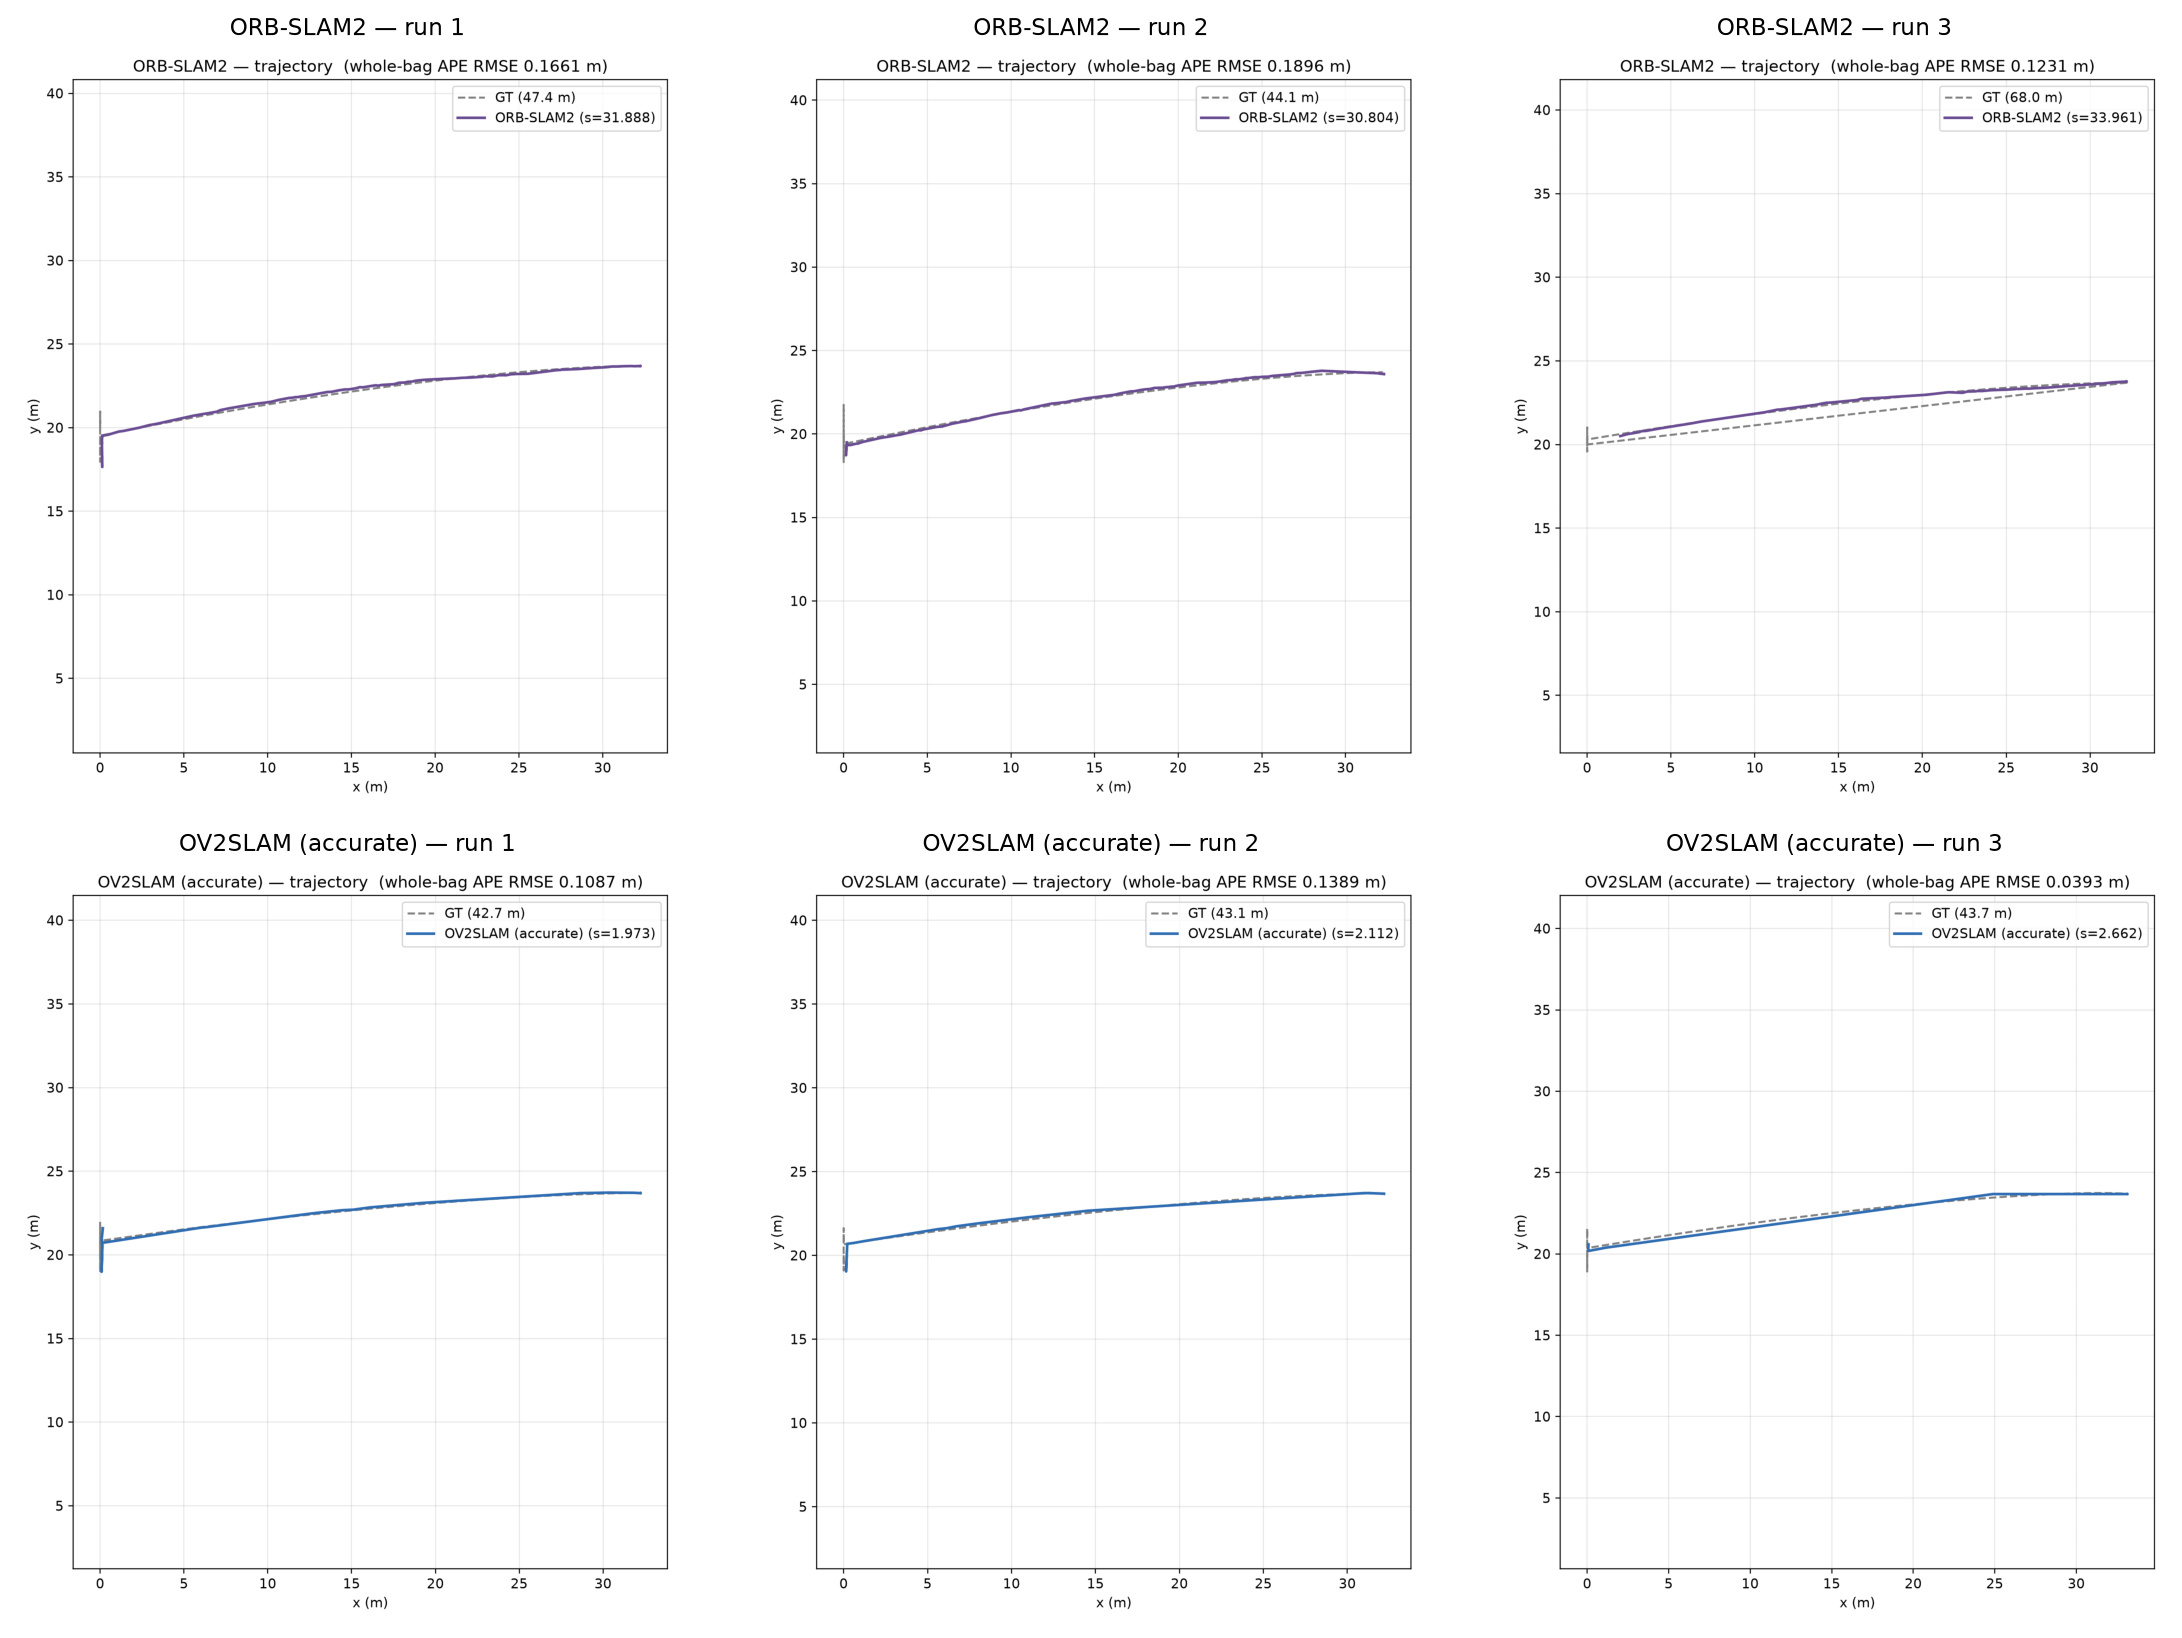
\includegraphics[width=\textwidth]{figures/cmp_trajectories_grid.png}
\caption{Top-down (x--y) ground-truth vs.\ SLAM trajectory overlay for all 6 runs
(whole bag, including the gate's pre-mission warm-up). Top row: ORB-SLAM2. Bottom
row: OV2SLAM (accurate). Dashed grey: ground truth. Solid: SLAM estimate
(Umeyama-aligned, scale $s$ shown in each legend). The short near-vertical
segment visible near the start of each trace is the gate's lateral warm-up
wiggle discussed in Section~2 -- not a plotting artifact.}
\label{fig:traj_grid}
\end{figure}

\section{Notes and Caveats}

\begin{itemize}
  \item n=3 runs per backend -- enough to see a consistent pattern, not enough
    for strong statistical claims.
  \item Only the \emph{accurate} OV2SLAM profile is represented here. The
    \emph{fast} profile has not yet completed a successful HIL run (its
    warm-up parallax fell short of OV2SLAM's initialization threshold in the
    one attempt made) -- see \texttt{docs/fixlog} for the diagnosis.
  \item ATE is computed against the \emph{online} \texttt{/slam/pose} stream
    (what the flight controller would consume live, had it been wired to SLAM
    -- see the boxed note in Section~1), not an offline, retroactively-optimized
    trajectory.
  \item Neither backend drives the flight in these 6 runs -- see the boxed note
    in Section~1.
  \item The OV2SLAM per-thread plot gap (Section~5) is the only known missing
    data point in this report; everything else reflects the 6 runs as recorded.
\end{itemize}

\end{document}
